\section{Chi tiết kỹ thuật}
\label{sec:chitiet}

\subsection{OCR hai độ phân giải và tách chú thích lề}

Bản hợp nhất có một cột chú thích hẹp ở lề phải ghi mỗi đoạn bắt nguồn từ văn bản gốc nào. Nếu
OCR cả trang một lượt, các chú thích này trộn vào giữa thân bài và phá vỡ cấu trúc. Giải pháp
là xử lý hai vùng riêng:

\begin{itemize}
  \item \textbf{Thân bài} dựng ở 300 DPI. Cột lề (từ 88,4\% chiều ngang trở đi) được
  \emph{xoá trắng} đúng những dải dọc có chú thích, chứ không xoá cả cột — vì một số dòng thân
  bài, như đoạn mở đầu trang 1, có tràn sang vùng đó.
  \item \textbf{Cột lề} dựng riêng ở 500 DPI vì chữ nhỏ hơn, rồi gom các dòng thành từng ghi
  chú theo khoảng cách dọc.
  \item \textbf{Khử bóng in ngược.} Bản quét hai mặt bị lộ chữ từ mặt sau; các điểm ảnh xám
  nhạt (trên ngưỡng 165) được đẩy về trắng trước khi nhận dạng.
  \item \textbf{Chuẩn hoá số.} OCR thường đọc nhầm “1” thành “l”, “I” hoặc “Ì”. Một bảng chuyển
  đổi sửa lại trước khi ghép thành chuỗi như \code{Khoản 1, Điều 2, TT17}; phần nào không chắc
  chắn được đánh dấu \code{?} để người rà soát để ý.
\end{itemize}

\subsection{Thuật toán phân mảnh}
\label{sec:chunk}

Đơn vị nhỏ nhất không bao giờ bị cắt là một \emph{block} (đoạn văn, mục gạch đầu dòng, hoặc cả
một bảng). Các block thuộc cùng một khoản tạo thành \emph{unit}; các unit thuộc cùng một
Điều/Phụ lục tạo thành một nhóm. Thuật toán đóng gói từng nhóm:

\begin{codeblock}
nếu tổng token của nhóm <= CHUNK_MAX_TOKENS:
    cả Điều là MỘT chunk                            <- trường hợp lý tưởng
ngược lại:
    gom các khoản liên tiếp cho tới sát ngưỡng
    nếu một khoản vẫn vượt ngưỡng:
        phần mở đầu ngắn (<= 150 token) được GÁN KÈM vào khoản dài phía sau
        cắt giữa các câu, chồng lấn CHUNK_OVERLAP_TOKENS
        các mảnh sau mảnh đầu được chèn lại dòng tiêu đề + " (tiếp)"
    không bao giờ kết thúc một chunk bằng một dòng tiêu đề trơ trọi
\end{codeblock}

Ba chi tiết đáng chú ý. \textbf{Thứ nhất}, câu bị ngắt bởi dấu sang trang được nối lại: nếu
block trước kết thúc không có dấu câu và block sau bắt đầu bằng chữ thường ở trang kế tiếp, hai
block được ghép. \textbf{Thứ hai}, câu dẫn vào bảng (“…được quy định như sau:”) được dính liền
với bảng, vì tách ra thì bảng mất đầu đề. \textbf{Thứ ba}, mỗi chunk mang một tiền tố ngữ cảnh
khi đem đi embed, nhưng tiền tố này \emph{không} nằm trong phần văn bản hiển thị cho người
dùng:

\begin{codeblock}
embed_text = "[Quy định học vụ ĐH (hợp nhất 2022) > Chương 2. PHƯƠNG THỨC ĐÀO TẠO
              > Điều 5. Thời gian đào tạo > 5.2 Thời gian đào tạo cụ thể]" + text
\end{codeblock}

Nhờ tiền tố này, một chunk nói về “8 học kỳ” vẫn tìm được bằng câu hỏi “thời gian đào tạo
chuẩn”, kể cả khi bản thân đoạn văn không chứa cụm đó.

\subsection{BM25 cho tiếng Việt}

Chỉ mục được xây theo \textbf{âm tiết và bigram âm tiết}: câu “đăng ký học phần” sinh ra các
term \code{đăng, ký, học, phần, đăng ký, ký học, học phần}. Bigram cho phép khớp cụm từ mà
không cần bộ tách từ tiếng Việt. Mỗi term được băm bằng BLAKE2b xuống chỉ số 31 bit; va chạm
băm hiếm và chỉ làm cộng dồn trọng số, không gây sai nghiêm trọng.

Trọng số lưu trong vector là phần tần suất của công thức BM25; thành phần IDF do Qdrant tự tính
nhờ cấu hình \code{modifier=IDF}, nên thêm văn bản mới không phải tính lại toàn kho. Tham số
\code{avgdl} được đo từ chính kho dữ liệu lúc nạp (372 âm tiết mỗi chunk) thay vì gán cứng —
con số gán cứng ban đầu là 400, lệch đáng kể và làm lệch phần chuẩn hoá độ dài.

\subsection{Mở rộng thuật ngữ}

Bảng tra gồm 38 từ viết tắt và 46 cụm thông dụng, ánh xạ sang đúng thuật ngữ trong quy định.
Cụm tương ứng được \emph{nối thêm} vào câu hỏi chứ không thay thế, nên ý gốc được giữ nguyên:

\begin{codeblock}
"GPA thấp bao nhiêu thì bị đuổi học?"
  -> "GPA thấp bao nhiêu thì bị đuổi học? — điểm trung bình tích luỹ; buộc thôi học"
\end{codeblock}

Ba cơ chế khớp. Viết tắt từ 3 ký tự trở lên khớp không phân biệt hoa thường; viết tắt 2 ký tự
(\code{TC}, \code{HK}, \code{HP}) bắt buộc viết hoa, để “tc” trong văn bản thường không bị hiểu
nhầm. Cụm thông dụng khớp không phân biệt hoa thường, ưu tiên cụm dài hơn (“bằng hai” thắng
“bằng”). Và khi phát hiện câu hỏi \textbf{không có dấu}, hệ thống đối chiếu bản không dấu của
câu hỏi với bản không dấu của bảng tra để khôi phục những cụm nhận ra được.

\subsection{Tra cứu trực tiếp theo số điều}

Khi câu hỏi gọi tên một điều khoản — “Điều 15 nói gì?”, “khoản 5.2 quy định sao?”, “phụ lục 7”
— ý định của người dùng là tường minh, và việc trông chờ hai vector đồng ý với nhau là thừa rủi
ro. Hệ thống nhận diện mẫu này bằng biểu thức chính quy (có xử lý số 0 đứng đầu và lỗi chính tả
dấu), rồi lấy thẳng các chunk của điều đó từ Qdrant qua bộ lọc payload, ghép vào danh sách ứng
viên. Các chunk này còn được cộng điểm thưởng lớn nhất trong bước rerank, và bỏ qua cả ngưỡng
liên quan.

\subsection{Hợp nhất có trọng số trong một round-trip}
\label{sec:fusion}

Phiên bản đầu dùng \code{FusionQuery(RRF)} của Qdrant. Vấn đề: RRF chỉ trả về điểm theo thứ
hạng, trong khi ngưỡng liên quan cần cosine thật — nên phải gọi Qdrant \emph{lần thứ hai} chỉ
để lấy lại cosine của đúng những điểm vừa tìm được. Hai round-trip cho một câu hỏi.

Phiên bản hiện tại gửi hai nhánh trong \textbf{một} request (\code{query\_batch\_points}), rồi
hợp nhất bằng Python:

\[
\mathrm{fused}(d) \;=\; \frac{w_{\text{dense}}}{60 + \mathrm{rank}_{\text{dense}}(d)}
\;+\; \frac{w_{\text{sparse}}}{60 + \mathrm{rank}_{\text{sparse}}(d)}
\]

với $w_{\text{dense}} = 1{,}0$ và $w_{\text{sparse}} = 0{,}8$ (dense được tin hơn một chút vì
các term BM25 bị băm). Điểm cosine và điểm BM25 gốc của từng nhánh được giữ nguyên trên mỗi ứng
viên, phục vụ ngưỡng liên quan, bộ rerank và trang chẩn đoán.

\subsection{Rerank heuristic}
\label{sec:rerank}

Bộ rerank chấm lại ứng viên bằng những tín hiệu mà tìm kiếm vector bỏ qua:

\begin{rtable}
\begin{tabular}{@{}p{0.32\textwidth} r p{0.47\textwidth}@{}}
\toprule
\textbf{Tín hiệu} & \textbf{Trọng số} & \textbf{Lý do} \\
\midrule
Điểm hợp nhất (chuẩn hoá) & 1,00 & Nền tảng, giữ kết quả của bước trước \\
Độ phủ từ khoá trong thân chunk & 0,45 & IDF cục bộ: từ có mặt ở mọi ứng viên thì không phân biệt được gì \\
Độ phủ trong tiêu đề Điều/Chương & 0,35 & “Điều 28. Phúc tra…” gần như chắc chắn trả lời câu hỏi về phúc tra \\
Câu hỏi gọi đúng số điều & 1,20 & Ý định tường minh phải thắng \\
Phạt trùng Điều (luỹ tiến) & $-0{,}18\,\tfrac{n(n+1)}{2}$ & Đoạn thứ hai cùng Điều vẫn cạnh tranh, đoạn thứ tư thì phải thật xuất sắc \\
\bottomrule
\end{tabular}
\captionof{table}{Tín hiệu và trọng số của bộ rerank heuristic.}
\label{tab:rerank}
\end{rtable}

\textbf{IDF cục bộ} là điểm mấu chốt: thay vì cần thống kê toàn kho, trọng số của một từ được
tính ngay trên tập ứng viên vừa lấy về, theo $\log\!\left(1 + \frac{n}{1+df}\right)$. Từ “sinh
viên” xuất hiện ở cả 20 ứng viên nên gần như không có trọng số; từ “phúc tra” xuất hiện ở một
ứng viên thì quyết định toàn bộ.

\begin{notebox}[title={Chi tiết dễ sai}]
Chuẩn hoá điểm phải \textbf{chia cho giá trị lớn nhất}, không dùng min–max. Min–max luôn ánh xạ
ứng viên tốt nhất về 1 và kém nhất về 0, nên hai ứng viên 0,51 và 0,50 trông xa nhau y như 1,0
và 0,0 — và khi đó không tín hiệu nào khác đủ sức lay chuyển thứ tự nữa. Lỗi này được phát hiện
nhờ một unit test, không phải nhờ đọc lại code.
\end{notebox}

\subsection{Mở rộng ngữ cảnh lân cận}

Câu trả lời của quy chế thường nằm vắt giữa hai khoản liền nhau: hỏi về số tín chỉ tối thiểu
thì khoản 15.3 nêu con số còn 15.4 nêu ngoại lệ. Sau khi chốt top-k, hệ thống lấy thêm tối đa 2
chunk lân cận trong cùng Điều và \textbf{xếp chúng xuống cuối} — vì \code{build\_context} cắt
theo ngân sách token từ cuối lên, nên phần bổ sung là thứ bị bỏ đầu tiên khi chật chỗ. Giao
diện đánh dấu riêng các đoạn này bằng nhãn “ngữ cảnh bổ sung”.

\subsection{Ngưỡng liên quan theo từng trích đoạn}
\label{sec:nguong}

Phiên bản đầu dùng ngưỡng liên quan như một cánh cổng chung: \emph{nếu có bất kỳ} ứng viên nào
vượt \code{MIN\_RELEVANCE\_SCORE} thì toàn bộ top-k được giữ. Hệ quả là mọi câu trả lời đều kèm
đúng \code{TOP\_K\_FINAL} “nguồn tham khảo” bất kể câu hỏi thật sự cần một hay năm, và một câu
hỏi không ai trả lời được vẫn dẫn ra năm trích đoạn — ngay trước khi mô hình tuyên bố nó không
tìm thấy gì.

Hiện tại mỗi trích đoạn phải tự vượt hai ngưỡng:

\[
\text{sàn} \;=\; \max\big(\text{\code{MIN\_RELEVANCE\_SCORE}},\;
\text{cosine}_{\max} \times \text{\code{RELATIVE\_CUTOFF}}\big)
\]

Ngưỡng tương đối là phần quan trọng. Cosine của \code{bge-m3} nằm trong một dải hẹp và cao —
một đoạn văn bất kỳ vẫn đạt khoảng 0,45 — nên chỉ riêng ngưỡng tuyệt đối không tách được đoạn
đúng khỏi đoạn đệm. Ngưỡng tương đối so sánh trong phạm vi chính lần tìm kiếm đó, nên nó thích
ứng theo từng câu hỏi.

Hai ngoại lệ có chủ ý: chunk được lấy vì câu hỏi gọi đích danh số điều thì giữ bất kể điểm, và
chunk chỉ do nhánh BM25 tìm ra thì không có cosine để chấm nên chỉ xét theo thứ hạng.
\code{TOP\_K\_FINAL} trở thành \emph{trần} chứ không phải định mức, và các chunk ngữ cảnh lân
cận chỉ lấp phần chỗ trống còn lại.

\begin{notebox}[title={Tham số phải đo, không đoán}]
\code{RELATIVE\_CUTOFF} siết quá tay sẽ loại nhầm Điều đúng. Nó không thể tinh chỉnh bằng bộ
test tự động, vì embedder giả dùng trong test có phân bố cosine trải rộng hơn \code{bge-m3}
nhiều nên cùng một tỉ lệ mang ý nghĩa khác. Harness vì vậy có chế độ \code{--sweep} chạy trên
hệ thống thật, in ra đường đánh đổi giữa số nguồn hiển thị và \code{hit@k}; quy tắc chọn là lấy
giá trị lớn nhất mà \code{hit@k} chưa suy giảm. Kết quả quét ở mục~\ref{sec:sweep}.
\end{notebox}

\subsection{Prompt}
\label{sec:prompt}

Prompt hệ thống ràng buộc sáu quy tắc: (1) chỉ dùng trích đoạn; (2) không đủ thông tin thì trả
lời đúng một câu cố định; (3) mỗi ý kèm trích dẫn lấy đúng tên văn bản và số Điều ghi ở đầu
trích đoạn; (4) giữ nguyên con số, mốc thời gian, điều kiện, và nêu rõ từng đối tượng nếu quy
định khác nhau; (5) ngắn gọn, dùng gạch đầu dòng khi nhiều ý; (6) không thêm dòng tóm tắt kiểu
“→ Đáp án: …”.

Quy tắc (2) là thứ làm cho việc từ chối trở nên \emph{phát hiện được}: câu trả lời chứa đúng
chuỗi đó thì hệ thống biết là không tìm được và không hiển thị nguồn. Quy tắc (6) cần thiết vì
mô hình nhỏ hay thêm dòng tóm tắt dù đã bị cấm; giao diện có thêm một lớp lọc chuỗi cho trường
hợp mô hình vẫn cố tình.

\subsection{Soát trích dẫn}

Sau khi mô hình viết xong, mọi cụm trong ngoặc vuông được phân tích để lấy ra số Điều/Phụ lục,
rồi đối chiếu với tập các Điều thực sự có trong ngữ cảnh. Những trích dẫn không có căn cứ được
trả về trong sự kiện \code{done} và giao diện tô màu cảnh báo. Hệ thống \textbf{không sửa} câu
trả lời — sửa tự động là thay một lỗi khó thấy bằng một lỗi khác khó thấy hơn; mục tiêu chỉ là
không để một con số bịa trông có vẻ đáng tin.

\subsection{Bảo vệ bước viết lại câu hỏi}
\label{sec:rewrite}

Câu hỏi nối tiếp phụ thuộc ngữ cảnh (“còn vừa làm vừa học thì sao?”) được viết lại thành câu
độc lập trước khi tra cứu. Cơ chế này có một chế độ hỏng nguy hiểm, phát hiện được trong quá
trình kiểm thử thực tế:

\begin{figure}[htbp]
\centering
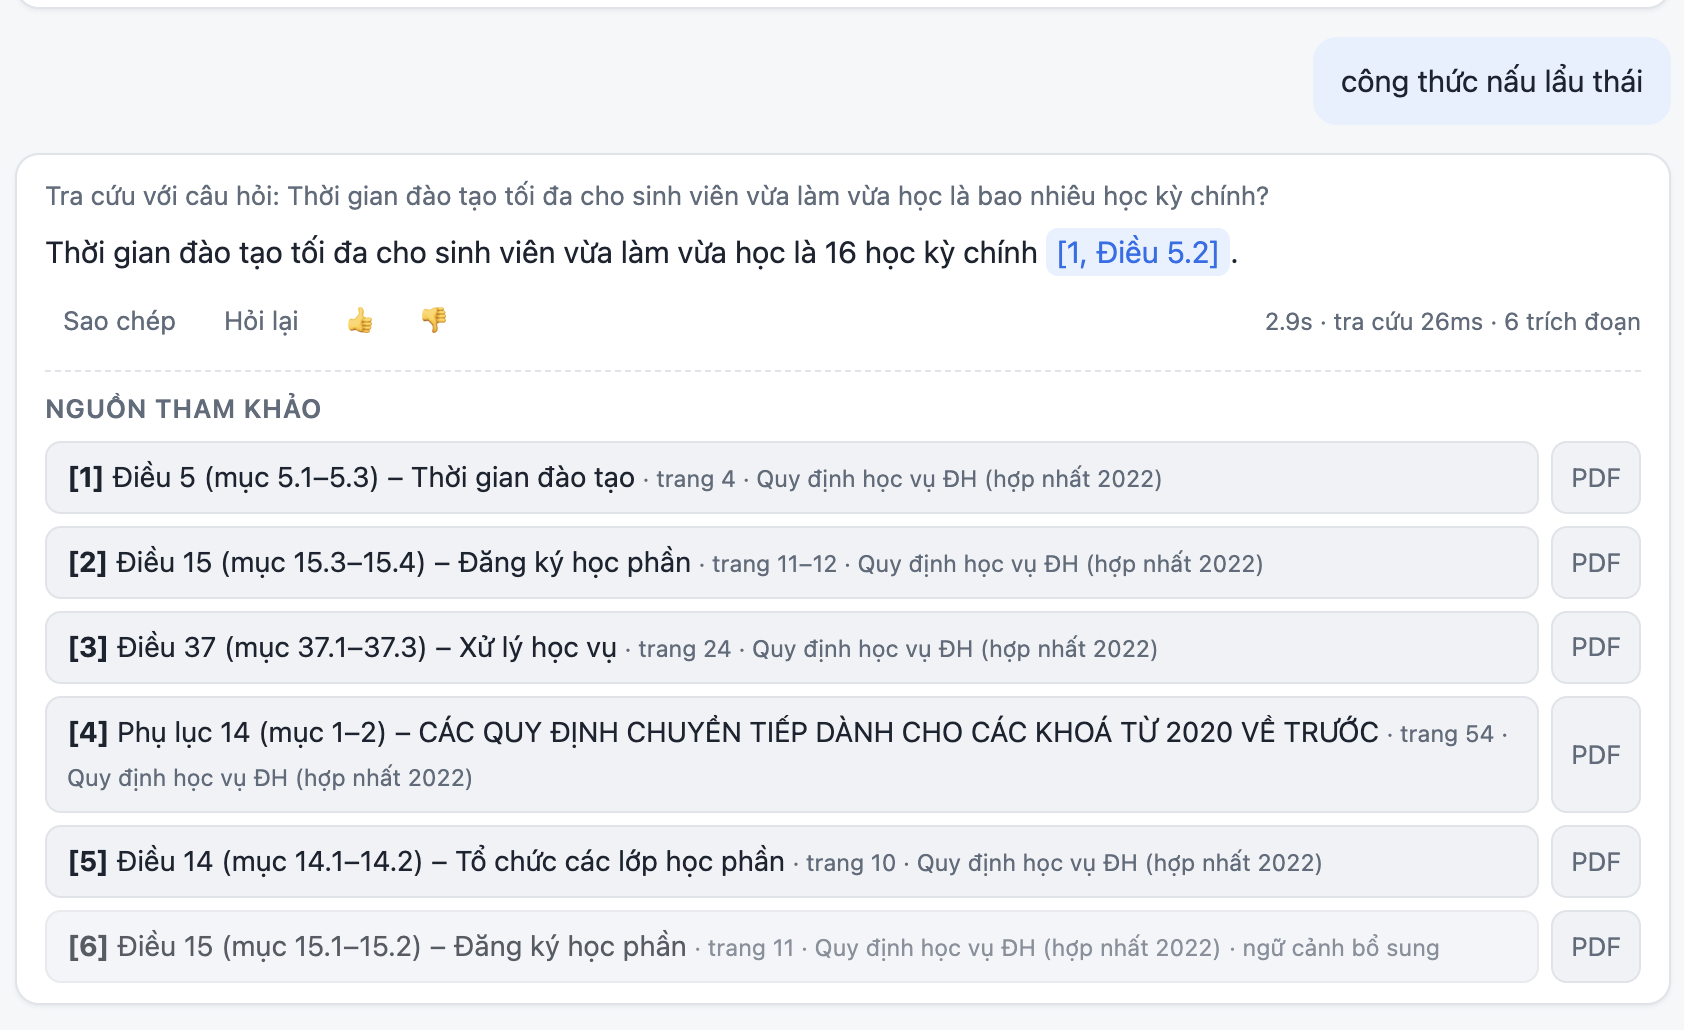
\includegraphics[width=0.88\textwidth]{img/bug-rewrite-hijack.png}
\caption{Chế độ hỏng đã được khắc phục: hỏi “công thức nấu lẩu thái” sau một lượt về thời gian
đào tạo, mô hình nhỏ trả về luôn \emph{câu hỏi trước} thay vì viết lại câu hỏi mới. Hệ quả là
câu trả lời sai chủ đề nhưng trích dẫn thật — dạng lỗi tệ nhất, vì mọi thứ phía sau đều trông
đúng.}
\label{fig:bug}
\end{figure}

Hai lớp khắc phục. Thứ nhất, ngưỡng kích hoạt được siết lại (dưới 5 từ thay vì dưới 6), nên một
câu hỏi ngắn nhưng tự đủ ý không còn bị viết lại. Thứ hai, và quan trọng hơn, kết quả viết lại
bị \textbf{kiểm tra trước khi dùng}: một bản viết lại hợp lệ luôn giữ lại ít nhất một từ nội
dung của câu hỏi gốc, vì bản chất của nó là bổ sung ngữ cảnh chứ không phải thay thế. Bản bị
cướp không giữ chữ nào của “lẩu thái” nên bị loại, hệ thống quay về câu hỏi gốc, và cơ chế
ngưỡng liên quan làm nốt phần việc từ chối.

\subsection{Nạp dữ liệu tăng dần}

Mã định danh chunk sinh bằng
\code{uuid5(doc\_id | article | index | sha256(body)[:16])} — tất định, nên nạp lại cùng một
nội dung sẽ ghi đè đúng điểm cũ chứ không nhân bản. Dấu vân tay mỗi văn bản gộp mã băm file,
phiên bản bộ phân mảnh, ngưỡng token, mô hình embedding, cờ hybrid và độ dài trung bình kho
(làm tròn theo bậc 50 âm tiết — nếu không, thêm một văn bản mới sẽ buộc nạp lại toàn bộ các văn
bản cũ chỉ vì trung bình xê dịch vài âm tiết).

\subsection{Các tối ưu độ trễ}
\label{sec:latency}

\begin{itemize}
  \item \textbf{Bỏ một round-trip Qdrant} (mục~\ref{sec:fusion}).
  \item \textbf{Bộ nhớ đệm vector câu hỏi.} Một lớp sinh viên hỏi gần như cùng vài chục câu;
  trên CPU mỗi lần embed tốn hàng chục mili-giây không cần lặp lại.
  \item \textbf{Bỏ bước viết lại khi không cần.} Trước đây \emph{mọi} câu hỏi nối tiếp đều tốn
  một lượt gọi LLM trước khi tìm kiếm.
  \item \textbf{Gửi trích đoạn trước câu trả lời.} Không làm hệ thống nhanh hơn, nhưng làm độ
  trễ \emph{cảm nhận được} ngắn hơn hẳn: người đọc có nội dung để đọc ngay.
  \item \textbf{Tắt chế độ suy luận của Qwen3} bằng \code{/no\_think}, kèm bộ lọc stream loại
  bỏ khối \code{<think>} kể cả khi thẻ bị cắt đôi giữa hai mẩu dữ liệu.
\end{itemize}

\chapterbreak
